\documentclass[10pt,a4paper]{article}

\usepackage[utf8]{inputenc}
%\usepackage[T1]{fontenc}
\usepackage{version}

\usepackage{amssymb,amsmath,amsthm}
\usepackage{graphicx}
\usepackage{enumerate}
\usepackage{tikz}
\usetikzlibrary{matrix,arrows}
\usepackage{todonotes}
\usepackage{fullpage}
\usepackage{hyperref}
\usepackage[french,linesnumbered,lined,boxed,commentsnumbered,ruled,vlined]{algorithm2e}

\renewcommand{\contentsname}{Table des matières}   

%\usepackage[ruled,vlined,linesnumbered,noresetcount]{algorithm2e}

\SetKwInput{KwIn}{Entrée}%
\SetKwInput{KwOut}{Sortie}%
%\SetKwIF{Si}{SinonSi}{Sinon}{si}{alors}{sinon si}{sinon}{fin si}%
%\SetKwFor{Tq}{tant que}{faire}{fin tq}%
%\SetKwFor{For}{Pour}

\usepackage{tikz}
\usetikzlibrary{positioning}
\usetikzlibrary{calc}

\usepackage[affil-it]{authblk}

\renewcommand*{\Authsep}{, }
\renewcommand*{\Authand}{, }
\renewcommand*{\Authands}{, }

\title{Projet de recherche sur l'article \textbf{Handling algebraic effects}\\
Résumer et mise en lien avec \textbf{erpl}}

\author[1]{Jordan Ischard}

\affil[1]{Université d'Orléans}

\date{}

% ===== ENVIRONMENTS ===== %
\newtheorem{theorem}{Théorème}
\newtheorem{lemma}{Lemme}
\newtheorem{corollary}[theorem]{Corollaire}
\newtheorem{claim}[theorem]{Claim}
\newtheorem{proposition}[theorem]{Proposition}
\newtheorem{definition}{Définition}
\theoremstyle{definition}
\newtheorem*{remark}{Remarque}
\newtheorem{exemple}{Exemple}

\newenvironment{proofclaim}{
	\noindent \emph{Proof.}
}{%
	\hfill $\diamond$ \\
}

% ===== COMMANDE POUR DEFINIR UN PROBLEME ===== %
\newcommand{\probleme}[4]{

    \vspace{0.4cm}
    \fbox{
        \begin{minipage}{0.95 \linewidth}
            \centerline{\textsc{\underline{#1}}}
            \textbf{Entr\'ee} : #2 \\ \textbf{#4} : #3
        \end{minipage}
    }
    \vspace{0.4cm}

}

\newcommand{\RMV}{\todo[inline]{Paragraphe à supprimer}}
\renewcommand*{\proofname}{Preuve}


\begin{document}

\maketitle
%\newpage
\tableofcontents
\newpage


\section*{Introduction}

	Le pionnier dans la gestion des effets algébriques est \textbf{Eugenio Moggi}. Il proposa une représentation uniforme de calcul d'effets grâce aux \textbf{Monades} \cite{DBLP:conf/ac/BentonHM00}. 
	Cette représentation est utilisé dans le langage \textbf{Haskell}.
	
	\begin{definition}
		Une \textbf{Monade} est une structure permettant de manipuler les langages fonctionnels purs
		avec des traits impératifs.
		On peut représenter une monade comme un triplet constitué de : 
		\begin{enumerate}
			\item un \textbf{constructeur de type} $\mathcal{M}$ appelé \textit{type monadique}, qui associe au type $\textbf{t}$ le type $\mathcal{M}\textbf{t}$.
			\item une \textbf{fonction} \verb|unit/return| qui construit à partir d'un élément de type 
			sous-jacent $\textbf{a}$ un autre élément de type monadique $\mathcal{M}\textbf{a}$. Cette fonction a la signature suivante : 
			
			\verb|unit/return|$~:~\textbf{t} \rightarrow \mathcal{M}\textbf{t}$.
			\item une \textbf{fonction $bind$}, représenté par l'opérateur infixe \verb|>>=|, associant à une valeur de type monadique
			et une fonction d'association une autre valeur de type monadique. Cette opérateur à la signature suivante : 
			
			\verb|>>=|$~:~\mathcal{M}\textbf{t} \rightarrow (\textbf{t} \rightarrow \mathcal{M}\textbf{u}) \rightarrow \mathcal{M}\textbf{u}$.
			
			L'idée derrière cette fonction est que l'on doit passé par un calcul pour accéder et traiter une valeur de type monadique afin de continuer le calcul.
		\end{enumerate}
	\end{definition}
	\bigbreak

	\begin{exemple} Voici un exemple de \textbf{Monade} trouvé sur le \href{http://lyah.haskell.fr/pour-une-poignee-de-monades}{site d'Haskell france}. On représente 
		une variable optionnelle.
		\begin{verbatim}
						-- Ici le constructeur de type est Maybe
						instance Monad Maybe where
						        -- La fonction qui construit notre type monadique
						        return x = Just x
						
						        -- La fonction bind qui nous permet de travailler avec le type monadique
				        Nothing >>= f = Nothing
						        Just x >>= f  = f x
								
						        -- Au cas où, une erreur se lève on dit qu'il n'y a rien
				        fail _ = Nothing
		\end{verbatim}
	\end{exemple}
	\bigbreak
	

	Les effets et leurs gestions sont utiles pour représenter les exceptions, les états mémoires, le non-déterminisme, les I/O, etc. \textbf{Moggi} ne fut pas le seul à proposer une gestion des effets, en effet \textbf{Plotkin et Power} proposerons plus tard une représentation basée sur un ensemble d'opérations qui représente la sources des effets et une théorie d'équations, pour ces dites opérations, qui décrit leurs propriétés.
	
	L'intuition derrière est que chaque calcul retourne soit une \textbf{valeur}, soit effectue une \textbf{opération} avec un retour déterminant la continuation. Les arguments de cette opération représente donc les potentiels continuations.
	
	\begin{exemple}
		On prend une opération binaire de choix \textbf{choose}. C'est une opération qui choisit de manière non déterministe un booléen à retourner :
		\[\textbf{choose(return true,return false)}\]
		
		On a deux possibilités : soit on continue avec le calcul donné par le première argument soit on continue avec le calcul donné par le second.
	\end{exemple}

	Les représentations respectives de \textbf{Moggi} et de \textbf{Plotkin et Power} permettent de gérer les effets et il est possible de passer d'une représentation à l'autre pour la plupart des effets. Typiquement les effets représentant les I/O et les états mémoires peuvent être exprimé dans les deux représentations. Les effets ayant cette caractéristique sont appelés \textbf{effets Algébriques}.
	\medbreak
	
	La vision algébrique des effets a permis de les combiner et de raisonner dessus. Cependant, le gestionnaire d'exception apporte un challenge.
	\smallbreak
	
	Soit la monade $\_ + \textbf{exc}$ pour l'ensemble des exceptions $\textbf{exc}$. Cette monade est représentée par une opération $\textbf{raise}_e()$ pour chaque $e \in \textbf{exc}$ et aucune équations. $\textbf{raise}_e()$ ne prend par d'arguments et il n'y a pas de continuation directement après une levée d'exception. Maintenant la monade défini, comment créer le gestionnaire d'exception ? L'approche commune est la suivante:
	\[\textbf{handle}_e(M,N)\]
		
	$M$ s'effectue à moins qu'une exception $e$ soit levée, dans ce cas on effectue $N$. Cette construction manque d'une certaine propriété caractérisant les opérations spécifiés dans les équations qui les décrivent.


	Dans l'article, une explication algébrique des gestionnaires d'exceptions est donné. L'idée principale est que :
	\begin{enumerate}
		\item les gestionnaires correspondent à des modèles de théorie équationnelle;
		\item la sémantique des gestionnaires est donné à l'aide d'homomorphismes uniques qui ciblent de tels modèles et est induit par la propriété universelle du modèle libre. 
	\end{enumerate}

	Il souhaite adopter une vision générale suggéré par Benton et Kennedy. Dans leur approche, la valeur de retour est passé à la continuation définit par l'utilisateur.
	Conceptuellement, les opérations algébriques et les gestionnaires d'effets sont duals, on a le \textit{constructeur d'effets} qui crée l'effet et le \textit{destructeur d'effets} qui produit un calcul en lien avec l'effet détruit.
	\smallbreak
	
	Le projet recherche a pour but de choisir un article et de le résumé. Mon résumé restera fidèle à l'article en gardant
	la forme du papier tout en allégeant le fond. En effet, il m'est plus important de montrer le concept général via des exemples ainsi
	que les résultats importants sur la validité des gestionnaires que d'expliquer la logique mathématique interne.

	De plus, le projet recherche étant lié à un autre module projet, je vais ajouter une plus-valu à mon résumé. Durant ma 
	1ère année de master, j'ai eu l'occasion d'implémenter une représentation des effets algébrique dans un noyau de langage fonctionnel créé lors de mon stage de fin de licence. Je vais donc profiter d'une section supplémentaire pour comparer les deux approches.
	
	

\section{Gestionnaire des exceptions}

On commence l'étude sur la gestionnaire des exceptions, d'une part pour comprendre le principe et d'autre part c'est un effet simple. La section est écrite de manière informelle.
\medbreak

On considère un ensemble fini d'exceptions $\textbf{exc}$, un second ensemble $A$ et une monade d'exception $TA$ telle que $TA \overset{\textbf{def}}{=} A + \textbf{exc}$. Un calcul retournant une valeur $a \in A$ est modélisé par un élément $ta \in TA$. Cette monade a pour unité $\eta_A : A \rightarrow A + \textbf{exc}$, et le calcul $return(V)$ est interprété par $\eta_A(V)$ tandis que $\textbf{raise}_e()$ est interprété par $in_2(e)$.

\subsection{Construction des gestionnaires étendus}

	Benton et Kennedy ont généralisé la construction des gestionnaires avec la forme suivante :
	\[M~\textbf{handled~with} \{\textbf{raise}_e() \mapsto N_e\}_{e \in \textbf{exc}}~\textbf{to}~ x:A.N(x)\]
	
	avec $\{...\}_{e \in \textbf{exc}}$ représentant l'ensemble des calculs, un pour chaque $e \in \textbf{exc}$. Dans cette construction, on effectue le calcul de $M \in A + \textbf{exc}$. Si on lève une exception $e \in \textbf{exc}$ alors on effectue un calcul $N_e$ qui retourne un élément de $B$ (où $B$ peut différer de $A$). Sachant que $N_e$ peut lui même lever une exception alors $N_e \in B + \textbf{exc}$. Les valeurs retournées par le gestionnaire sont passées dans une continuation défini par l'utilisateur $N : A \rightarrow B + \textbf{exc}$. La construction satisfait 2 équations :
	\begin{align*}
		\textbf{return} ~V~\textbf{handled~with} \{\textbf{raise}_e() \mapsto N_e\}_{e \in \textbf{exc}}~\textbf{to}~ x:A.N(x) &= N(V)\\
		\textbf{raise}_{e'}()~\textbf{handled~with} \{\textbf{raise}_e() \mapsto N_e\}_{e \in \textbf{exc}}~\textbf{to}~ x:A.N(x) &= N_{e'}
	\end{align*}
	
	Comme discuté dans \cite{DBLP:journals/jfp/BentonK01}, Cette construction permet d'écrire de façon simple un idiome de programmation qui était lourd à mettre en place. 
	\smallbreak
	Algébriquement le calcul $N_e$ donne un nouveau modèle $\mathcal{M}$ pour la théorie des exceptions. Le porteur de ce modèle est $B + \textbf{exc}$. Pour chaque $e \in \textbf{exc}$, $\textbf{raise}_e()$ est interprété par $N_e$. On peut voir d'après les deux équations ci-dessus que :
	\[h(M) \overset{def}{=} M~\textbf{handled~with} \{\textbf{raise}_e() \mapsto N_e\}_{e \in \textbf{exc}}~\textbf{to}~ x:A.N(x)\]
	
	où $h : A + \textbf{exc} \rightarrow \mathcal{M}$ est l'homomorphisme unique qui étend $N$, i.e, tel que l'on a le diagramme de commutation suivant : 
	
	\begin{center}
		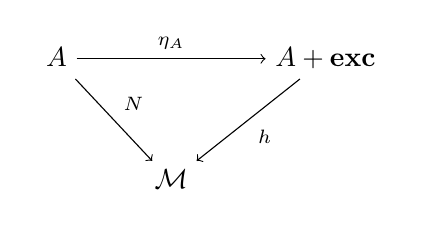
\begin{tikzpicture}[description/.style={fill=white,inner sep=2pt}]
		\matrix (m) [matrix of math nodes, row sep=3em,
		column sep=2.5em, text height=1.5ex, text depth=0.25ex]
		{ A & & A + \textbf{exc} \\
			& \mathcal{M} & \\ };
		\path[->,font=\scriptsize]
		(m-1-1) edge node[auto] {$ \eta_A$} (m-1-3)
		edge node[auto] {$ N $} (m-2-2)
		(m-1-3) edge node[auto] {$ h $} (m-2-2);
		\end{tikzpicture}
	\end{center}
	
	Notons que tous les homomorphismes d'un modèle libre vers un modèle pour un porteur donné sont obtenus de cette manière. Donc la construction proposé par Benton et Kennedy est le plus général possible d'un point de vue algébrique.

	\subsection{Gestion des effets algébriques arbitraires}
	
	Avec la construction étendue de Benton et Kennedy, on voit maintenant comment créer les gestionnaires pour les autres effets algébriques. Un \textbf{modèle d'une théorie d'équations} est une interprétation, i.e, un ensemble de tableaux associatifs, un pour chaque opération, qui satisfont les équations. Les gestionnaires permettent de telles interprétations. Comme avant, les calculs sont interprétés par le modèle libre et la construction des gestionnaires sont interprétés par l'homomorphisme induit. Avant, les exceptions étaient remplacés par un calcul du gestionnaire; maintenant les \textbf{opérations} sont remplacées par les tableaux associatifs du gestionnaire.
	\smallbreak
	Il est important de noter que toute interprétation ne donne pas forcément un modèle de la théorie des équations et que donc tous les gestionnaires ne sont pas forcément correctes. Plus que ça, la validité d'un gestionnaire peut être indéfini. Pour contourner le problème, il y a deux écoles. Soit on contraint l'utilisateur à des gestionnaires prédéfinies que l'on sait correcte; soit on laisse une totale liberté à l'utilisateur mais c'est à lui qui est responsable de la validité de ses gestionnaires. On adoptera la seconde dans ce papier.
	
	
\newpage
\section{Syntaxe}

\subsection{Signatures}

	Les types de signature $\alpha,\beta$ sont définis par:
	\[\alpha,\beta := \textbf{b}~|~\textbf{1}~|~\alpha \times \beta~|~\sum_{l \in L}\alpha_l\]
			
	où \textbf{b} représente l'ensemble des types de base, $L$ représente un sous-ensemble fini de label. On ne spécifie pas l'ensemble $L$ mais on assume que les labels que l'on va utiliser seront disponibles. Cependant, on spécifie un sous-ensemble de \textbf{b} comme un \textbf{type de base d'arité} ce qui nous permet d'introduire la définition suivante : 
	
	\begin{definition}
		Un type de signature est un type de signature \textbf{d'arité} si et seulement si tous les types de base qu'il contient sont des types de base d'arité.
	\end{definition}
	
	Les ensembles finis peuvent être représentés par le type de signature $\sum_{l \in L}\alpha_l$ et les ensembles infinis sont représentés par le type de base correspondant.
	
	\begin{exemple}
		On peut représenter les booléens par  $\sum_{bool \in \{true,false\}} \textbf{1}$ et un sous-ensemble d'entier par $\sum_{n \in \{1,...,m\}}\textbf{1}$.
	\end{exemple}
	\bigbreak


	On définit les symboles de fonctions typés par : $\textbf{f} : \alpha \rightarrow \beta$. Ils représentent les fonctions prédéfinies, telles que $+ : \textbf{nat} \times \textbf{nat} \rightarrow \textbf{nat}$ ou encore $< : \textbf{nat} \times \textbf{nat} \rightarrow \textbf{bool}$.
	\medbreak

	Pour finir, on définit les symboles d'opérations typés par : $\textbf{op} : \alpha \rightarrow \beta$, tels que chaque $\beta$ est un type de signature d'arité et tels que $\textbf{op}$ a une théorie d'effet $\tau$. Les opérations deviennent la source des effets et la théorie d'effet indique leurs propriétés.
	


	On interprète $\textbf{op} : \alpha \rightarrow \beta$ de la façon suivante :
	$\textbf{op}$ accepte un paramètre $\alpha$ et après avoir exécuté l'effet approprié, son type de retour $\beta$ détermine la continuation.
	\medbreak
	
	Maintenant que tout est définis, on peut créer une signature. Le choix de la signature va dépendre de ce que l'on veut représenter.

	\begin{exemple}\label{exStateExc}
		On présente quelques exemples prit de \cite{DBLP:journals/tcs/HylandPP06}.
		\begin{enumerate}
			\item[]\textbf{Exceptions} : On prend l'unique symbole d'opération $\textbf{raise} : \textbf{exc} \rightarrow \textbf{0}$ paramétré sur l'ensemble \textbf{exc} afin de lever une exception. Le symbole de l'opération est nul (\textbf{0}) car il n'y a pas de continuation après une levée d'exception. Il faut donc gérer les exceptions.
			
			\item[]\textbf{State} : On prend le type de base d'arité \textbf{nat} (qui représente l'ensemble des naturelles), le type de base d'arité \textbf{loc} (un ensemble fini d'emplacement) et les symboles d'opérations $\textbf{get} : \textbf{loc} \rightarrow \textbf{nat}$ et $\textbf{set} : \textbf{loc} \times \textbf{nat} \rightarrow \textbf{1}$. On part du principe que l'on stocke des naturelles dans des emplacements mémoire, \textbf{get} permet de récupérer le naturelle pour un emplacement donné tandis que \textbf{set} remplace l'élément à l'emplacement donné en paramètre par le second élément donné en paramètre et ne retourne rien. 
		\end{enumerate}
	\end{exemple}

\subsection{Types}
	
	Le langage que l'on définit suit l'approche \textit{call-by-push-value} de Levy \cite{DBLP:journals/lisp/Levy06}. On a donc une séparation stricte entre les valeurs et les calculs. Ces types sont donnés par : 
	\begin{align*}
		A,B &:= \textbf{b}~|~\textbf{1}~|~A \times B~|~\sum_{l \in L} A_l~|~U\underline{C}\\
		\underline{C} &:= FA~|~\Pi_{l\in L}~\underline{C}_l~|~A \rightarrow\underline{C}
	\end{align*}
	
	Les types de valeur étendent les types de signature en ajoutant le constructeur de type $U\_$. Le type $U\underline{C}$ représente les types de calcul $\underline{C}$ qui ont été bloqué dans une valeur. Le calcul pourra être forcé plus tard.
	
	$FA$ représente les calculs qui retourne une valeur de type $A$. La fonction $A \rightarrow \underline{C}$ représente les calculs de type $\underline{C}$ nécessitant un paramètre de type $A$. Pour finir, le type de calcul produit $\Pi_{l\in L} \underline{C}_l$ représente un ensemble fini indexé de calcul produit de type $\underline{C}_l$, pour $l \in L$. Ces tuples ne sont pas évalués de façon séquentiel comme dans la stratégie d'évaluation \textit{call-by-value}. À la place, un composant d'un tuple est évalué seulement une fois qu'il a été sélectionné via une projection. 
	
\subsection{Termes}

	On a définit les signatures et les types, il nous manque les termes. On va les définir en trois parties : les termes \textbf{valeur} $V,W$, les termes \textbf{calcul} $M,N$ et les termes \textbf{gestionnaire} $H$. Ils sont définit par :
	\begin{align*}
		V,W :=&~x~|~f(V)~|~\langle\rangle~|~\langle V,W\rangle~|~l(V)~|~\textbf{thunk}~M\\
		M,N :=&~\textbf{match}~V~\textbf{with}~\langle x,y\rangle  \mapsto M~|~\textbf{match}~V~\textbf{with}~\{l(x_l)  \mapsto M_l\}_{l \in L}~|~\textbf{force}~V~|\\
		&~\textbf{return}~V~|~M~\textbf{to}~x:A.N~|~\langle M_l\rangle_{l \in L}~|~\textbf{prj}_l~M~|~\lambda x:A.M~|~M~V~|~k(V)~|\\
		&~\textbf{op}_V(x:\beta .M)~|~M~\textbf{handled}~\textbf{with}~H~\textbf{to}~x:A.N\\
		H :=&~\{\textbf{op}_{x:\alpha}(k:\beta \rightarrow \underline{C}) \mapsto M_\textbf{op} \}_{\textbf{op}:\alpha \rightarrow \beta}
	\end{align*}
	
	avec $x,y$ appartenant à l'ensemble des variables de valeur et $k$ appartenant à l'ensemble des variables de continuation. $\{...\}_{l \in L}$ représente l'ensemble des calculs, un pour chaque $l \in L$. Même principe pour $\{...\}_{\textbf{op} : \alpha \rightarrow \beta}$.

	La syntaxe respecte celle présenté avec l'approche \textit{call-by-push-value} excepté pour la partie gestionnaire et la dernière ligne des termes \textbf{calcul}.
	\smallbreak
	
	On a le terme d'une \textit{application d'opération}
		\[\textbf{op}_V(x:\beta .M)\]
	
	 Elle fonctionne de la manière suivante : l'opération \textbf{op} paramétré par $V$ est effectuée, ensuite on affecte le résultat à $x$ et enfin on évalue la continuation $M$.

	\begin{exemple}\label{get1}
		Le calcul suivant incrémente le nombre $n$, le stocke dans l'emplacement $l$ et retourne l'ancienne valeur.
		\[\textbf{get}_l(n:\textbf{nat}.\textbf{set}_{\langle l,n+1\rangle}(x:\textbf{1}.\textbf{return~n}))\]
	\end{exemple}
	\bigbreak
	
	Ensuite, le terme du gestionnaire
		\[\{\textbf{op}_{x:\alpha}(k:\beta \rightarrow \underline{C}) \mapsto M_\textbf{op} \}_{\textbf{op}:\alpha \rightarrow \beta}\]
		
	est définit par un ensemble fini de définitions d'opérations qui gère les effets 
		\[\textbf{op}_{x:\alpha}(k:\beta \rightarrow \underline{C}) \mapsto M_\textbf{op}\]
			
	une pour chaque \textbf{op}. Le terme gestionnaire $M_\textbf{op}$ est dépendant de la variable $x$ et de la continuation $k$. À noter que $k$ sera toujours utiliser de la manière suivante : $k(V)$ ou $V$ est la valeur appliqué à la continuation.
	
	\begin{exemple}\label{get2}
		Bien que l'on ne peut pas modifier une valeur en lecture-seule (c'est un cas spécifique ou on ne peut pas utiliser l'opération \textbf{set}), il est tout de même possible d'évaluer un calcul avec une valeur temporairement modifiée. Pour faire cela, on crée un gestionnaire \textit{état-temporaire} qui dépend d'une variable $n$ (la dite variable temporaire) :
		\[H_{temporary} = \{\textbf{get}_{l:\textbf{loc}}(k:\textbf{nat} \rightarrow \underline{C}) \mapsto k(n)\}\]

	\end{exemple}

	Finalement, on a le terme de calcul \textit{gestionnaire}
		\[M~\textbf{handled}~\textbf{with}~H~\textbf{to}~x:A.N\]		

	Il évalue $M$, gérant tous les calculs d'opérations grâce à $H$. Ensuite il associe le résultat à $x$ et enfin évalue $N$. C'est un point clé pour la compréhension de l'article, on va donc détailler. 
	
	On suppose que $M$ veut effectuer une opération $\textbf{op}_V(y.M')$ correspondant au terme de gérant $\textbf{op}_z(k) \mapsto M_\textbf{op} \in H$. On substitue l'évaluation de \textbf{op} par $M_\textbf{op}$ en associant $z$ avec $V$ et en remplaçant la continuation $k(W)$ pour chaque occurrence de celle-ci dans $M_\textbf{op}$ avec 
		\[M'[W/y]~\textbf{handled}~\textbf{with}~H~\textbf{to}~x:A.N\]

	La continuation $k$ reçoit la valeur $W$ déterminé par $M_\textbf{op}$. Elle est ensuite géré de la même façon que $M$, ce qui n'est pas le cas de $M_\textbf{op}$. En effet $M_\textbf{op}$ n'est pas géré par $H$, donc ses opérations échappent à $H$ mais peuvent cependant être gérées par un autre gestionnaire imbriqué. 
	
	\begin{exemple}\label{get3}
		On considère le gestionnaire d'état temporaire $H_{temporary}$ donné dans Exemple \ref{get2}. On prend la calcul suivant :
		\begin{align*}
			& \textbf{let}~n:\textbf{nat}~\textbf{be}~20~\textbf{in}\\
			& \textbf{get}_l(x:\textbf{nat}.get_l(y:\textbf{nat}.\textbf{return}~x+y))\\
			&\textbf{handled~with}~H_{temporary}~\textbf{to}~z:A.\textbf{return}~z+2
		\end{align*}
	
	Dans ce calcul on va associer $n$ avec la valeur $20$. Le premier \textbf{get} va être géré par $H_{temporary}$ et va donc associer $x$ avec la valeur de $n$ donc $20$. Le second \textbf{get} appartient à la continuation et est donc géré aussi par $H_{temporary}$, i.e, il va associer $y$ avec $20$ (par la même logique que le premier \textbf{get}). On retourne $x + y$ donc $20 + 20$ soit $40$ et on associe ce résultat à $z$. On retournera au final $42$.
	\end{exemple}
	
\subsection{Jugement de types}

	Tous les jugements de types sont fait dans le contexte de valeurs
		\[\Gamma = x_1:A_1,...,x_m:A_m\]
		
	avec les variables de valeurs $x_i$ associées à un type de valeurs $A_i$ et dans le contexte de continuations
		\[K = k_1:\alpha_1 \rightarrow \underline{C}_1,...,k_n:\alpha_n \rightarrow \underline{C}_n\]
		
	avec les variables $k_j$ associées à un type de continuation $\alpha_j \rightarrow \underline{C}_j$. 
	\bigbreak
	Les valeurs sont typés par $\Gamma~|~K \vdash V:A$, ensuite les calculs sont typés par $\Gamma~|~K \vdash M:\underline{C}$ et enfin les gestionnaires sont typés par $\Gamma~|~K \vdash H:\underline{C}~\textbf{handler}$.
	\smallbreak 
	Les valeurs sont typés en suivant les règles ci-dessous : 
	\begin{align*}
		&\Gamma~|~K \vdash x:A~(x:A \in \Gamma) & &\dfrac{\Gamma~|~K \vdash V:\alpha}{\Gamma~|~K \vdash f(V):\beta}~(\textbf{f}:\alpha \rightarrow \beta) & &\dfrac{\Gamma~|~K \vdash M:\underline{C}}{\Gamma~|~K \vdash \textbf{thunk}~M:U\underline{C}}\\\\
		&\dfrac{\Gamma~|~K \vdash V:A\quad\quad\Gamma~|~K \vdash W:B}{\Gamma~|~K \vdash \langle V,W \rangle:A \times B} & &\dfrac{\Gamma~|~K \vdash V:A_l}{\Gamma~|~K \vdash l(V):\sum_{l \in L}A_l}~(l \in L) & &\Gamma~|~K \vdash \langle\rangle:\textbf{1}
	\end{align*}
	
	Les calculs sont typés en suivant les règles ci-dessous :
	\[\dfrac{\Gamma~|~K \vdash V : A \times B\quad\quad\Gamma~x:A,y:B~|~K \vdash M:\underline{C}}{\Gamma~|~K \vdash \textbf{match}~V~\textbf{with}~\langle x,y\rangle  \mapsto M:\underline{C}}\]
	\begin{align*}	
		&\dfrac{\Gamma~|~K \vdash V : \sum_{l \in L}A_l\quad\quad\Gamma~,x_l:A_l~|~K \vdash M_l:\underline{C}~~(l\in L)}{\Gamma~|~K \vdash \textbf{match}~V~\textbf{with}~\{ l(x_l) \mapsto M_l\}_{l \in L}:\underline{C}} &
		&\dfrac{\Gamma~|~K \vdash V : U\underline{C}}{\Gamma~|~K \vdash \textbf{force}~V:\underline{C}}\\\\
		&\dfrac{\Gamma~|~K \vdash M:FA\quad\quad\Gamma,x:A~|~K \vdash N:\underline{C}}{\Gamma~|~K \vdash M~\textbf{to}~x:A.N:\underline{C}} &
		&\dfrac{\Gamma~|~K \vdash V : A}{\Gamma~|~K \vdash \textbf{return}~V:FA}\\\\
		&\dfrac{\Gamma~|~K \vdash V:\alpha\quad\quad\Gamma,x:\beta~|~K \vdash M : \underline{C}}{\Gamma~|~K \vdash \textbf{op}_V(x:\beta.M):\underline{C}}~~(\textbf{op}:\alpha \rightarrow \beta) &
		&\dfrac{\Gamma~|~K \vdash M : \Pi_{l\in L} \underline{C}_l}{\Gamma~|~K \vdash prj~M:\underline{C}_l}~~(l \in L) \\\\
		&\dfrac{\Gamma~|~K \vdash M : A \rightarrow \underline{C}\quad\quad\Gamma~|~K \vdash V:A }{\Gamma~|~K \vdash M~V:\underline{C}  } &
		&\dfrac{\Gamma,x:A~|~K \vdash M : \underline{C}}{\Gamma~|~K \vdash \lambda x:A.M:A \rightarrow \underline{C}} \\\\
		&\dfrac{\Gamma~|~K \vdash V:\alpha}{\Gamma~|~K \vdash k(V):\underline{C}}~~(k:\alpha \rightarrow \underline{C} \in K) &
		&\dfrac{\Gamma~|~K \vdash M_l:\underline{C}_l~~(l \in L)}{\Gamma~|~K \vdash \langle M_l\rangle_{l \in L}:\Pi_{l\in L}\underline{C}_l}\\
	\end{align*}
	\[\dfrac{\Gamma~|~K \vdash M:FA\quad\quad\Gamma~|~K \vdash H : \underline{C}~\textbf{handler}\quad\quad\Gamma,x:A~|~K \vdash N:\underline{C}}{\Gamma~|~K \vdash M~\textbf{handled}~\textbf{with}~H~\textbf{to}~x:A.N : \underline{C}}\]	
	
	
	Les gestionnaires sont typés en suivant la règle ci-dessous : 
	\begin{align*}
		\dfrac{\Gamma,x:\alpha~|~K,k:\beta \rightarrow \underline{C} \vdash M_\textbf{op}:\underline{C}~~(\textbf{op}: \alpha \rightarrow \beta)}{\Gamma~|~K \vdash \{\textbf{op}_{x : \alpha}(k:\beta \rightarrow \underline{C}) \mapsto M_\textbf{op}\}_{\textbf{op}:\alpha \rightarrow \beta}:\underline{C}~\textbf{handler}}
	\end{align*}

	À partir de maintenant, on utilisera une succession d'abréviations décrite en Annexe.
	\medbreak
	
	\begin{definition}\label{fctnOp}
		Quand un gestionnaire contient des termes gérant uniquement un sous-ensemble $\Theta$ de symbole d'opérations, on assume que les symboles d'opérations restants sont gérés par "eux-même". De façon plus formel, on va définir le gestionnaire tel que :
		
		
		\begin{center}
			$ \{\textbf{op}_x(k) \mapsto M_\textbf{op}\}_{\textbf{op} \in \Theta} \overset{def}{=}
			\left \{ \textbf{op}_x(k) \mapsto
			\left \{ 
			\begin{array}{lr}
			M_\textbf{op}&(\textbf{op} \in \Theta) \\
			\textbf{op}_x(y:\beta.k(y))&(\textbf{op} \notin \Theta)
			\end{array}
			\right \}
			\right .
			_\textbf{op}$ 
		\end{center}
	\end{definition}




\newpage
\section{Exemples}
%On va montrer à travers une succession d'exemples la portée des gestionnaires d'effets algébriques. La notion de validité des exemples est traitée plus loin dans le résumé.

\subsection{Non-déterminisme explicite}

	L'évaluation d'un calcul non-déterminisme prend habituellement un seul chemin possible. Une alternative est de prendre tous les chemins possibles et d'autoriser qu'un chemin échoue. Le second choix va être représenté dans la syntaxe du langage.
	%On utilisera cette alternative comme en Haskell. 
	Pour cela, Le symbole d'opération \textbf{fail} est ajouté afin de représenter les chemins qui échouent.
	
	On considère un gestionnaire qui introduit le résultat d'un calcul dans une liste. Les listes de types basiques \textbf{b} sont définit par le symbole $\textbf{list}_\textbf{b}$. Ainsi que les symboles de fonctions: 
	$\textbf{nil} : \textbf{1} \rightarrow \textbf{list}_\textbf{b}$, 
	$\textbf{cons}: \textbf{b} \times \textbf{list}_\textbf{b} \rightarrow \textbf{list}_\textbf{b}$ et $\textbf{append} : \textbf{list}_\textbf{b} \times \textbf{list}_\textbf{b} \rightarrow \textbf{list}_\textbf{b}$.
	\smallbreak
	
	On définit un calcul qui pour tout élément de type \textbf{b} retourne un élément de type $\textbf{list}_\textbf{b}$ tel que : 
	\[\Gamma~|~K~\vdash~M~\textbf{handled~with}~H_{list}~\textbf{to}~x:\textbf{b}.\textbf{return~cons}(x,\textbf{nil}):F\textbf{list}_\textbf{b}\]

	avec $H_{list}$ définit par :
	\begin{align*}
		\Gamma~|~K~\vdash~\{& \\
		 &\textbf{fail}() \mapsto \textbf{return~nil},\\
		 &\textbf{choose}(k_1,k_2) \mapsto k_1~\textbf{to}~l_1:\textbf{list}_\textbf{b}.k_2~\textbf{to}~l_2:\textbf{list}_\textbf{b}.\textbf{return}~\textbf{append}(l_1,l_2) \\
		 &\}:F\textbf{list}_\textbf{b}~\textbf{handler}
	\end{align*}

	Voyons comment le gestionnaire fonctionne. 
	\begin{enumerate}
		\item[(1)] On considère que $M$ contient un symbole d'opération \textbf{choose}. Lorsque l'on va évaluer l'opération $\textbf{choose}(x,y)$, on va regarder si $M$ est géré. Ici, on a $H_{list}$. Ensuite on va voir dans $H_{list}$ si \textbf{choose} est géré. C'est le cas, on va donc calculer 
		\[M_\textbf{choose} [x/k1,y/k2] = (k_1~\textbf{to}~l_1:\textbf{list}_\textbf{b}.k_2~\textbf{to}~l_2:\textbf{list}_\textbf{b}.\textbf{return}~\textbf{append}(l_1,l_2))[x/k1,y/k2]\]
		
		Deux choses à noter : la continuation n'est pas utilisé dans $M_\textbf{choose}$; on part du principe que les continuations $k_1$ et $k_2$ retourne un élément de type $\textbf{list}_\textbf{b}$.
		
		\item[(2)]On considère que $M$ contient un symbole d'opération \textbf{fail}. En suivant la même logique que ci-dessus, On va calculer
		\[M_\textbf{fail} = \textbf{return~nil}\]
		
		Une fois encore la continuation n'est pas gardé. Il est important de noter qu'un chemin invalide retourne aussi un élément de type $\textbf{list}_\textbf{b}$.
	\end{enumerate}
\subsection{Timeout}

	Le gestionnaire du \textit{timeout} donne un exemple de paramètre passé dans la continuation. On souhaite effectuer un calcul et attendre pour un certains temps donné. Si le calcul n'est pas compléter avant le temps donné alors on retourne une valeur par défaut. On représente le temps via une seule opération $\textbf{delay} : \textbf{nat} \rightarrow \textbf{1}$, telle que $\textbf{delay}_t(M)$ est le calcul qui attend un temps $t$ et ensuite effectue le calcul $M$. Pour tout type $A$, on a le gestionnaire $H_{timeout}$ suivant: 
	\begin{align*}
		\Gamma,x_0:A,t_{wait}:\textbf{nat}~|~K~\vdash~\{& \\
		&\textbf{delay}_t(k:\textbf{nat} \rightarrow FA) \mapsto \lambda t_{spent} :\textbf{nat}.\\
		&\textbf{if}~t+t_{spent} \leq t_{wait}\\
		&\quad\textbf{then}~\textbf{delay}_t(k(t+t_{spent})~t_{spent})\\
		&\quad\textbf{else}~\textbf{delay}_{t_{wait} - t_{spent}}(\textbf{return}~x_0) \\
		&\}:\textbf{nat} \rightarrow FA~\textbf{handler}
	\end{align*}
	\newpage
	
	Le terme qui gère \textbf{delay} (que l'on va nommé $M_\textbf{delay}$) dépend de la variable $t_{spent}$, qui représente le temps que l'on a déjà attendu.
	Si l'on souhaite utiliser ce gestionnaire, on va devoir lui spécifier un paramètre initial. On veut gérer $M:FA$ via $H_{timeout}$ or on a le calcul suivant :
	\[\Gamma,x_0:A,t_{wait}:\textbf{nat}~|~K~\vdash~M~\textbf{handled~with}~H_{timeout}~\textbf{to}~x:A.\lambda t:\textbf{nat}.\textbf{return}~x:\textbf{nat} \rightarrow FA\]
	
	Le calcul géré est de type $\textbf{nat} \rightarrow FA$, on voit la nécessité du paramètre initial pour passer à un calcul géré de type $FA$.
	\[\Gamma,x_0:A,t_{wait}:\textbf{nat}~|~K~\vdash~(M~\textbf{handled~with}~H_{timeout}~\textbf{to}~x:A.\lambda t:\textbf{nat}.\textbf{return}~x)~0:FA\]
	
	il est nécessaire d'ajouter une abstraction autour de $\textbf{return}~x$ car si on suppose que $M$ ne contient pas de symbole d'opération $\textbf{delay}$ alors on aura le calcul suivant : $(\lambda t:\textbf{nat}.\textbf{return}~x)~0:FA$. 
	\bigbreak
	
	\begin{exemple}
		On effectue le calcul ci-dessous avec $M = \textbf{delay}_5(t_2.(\textbf{return}~t_2 + 45))$ (on symbolisera le passage d'une étape de calcul via le symbole $\Rightarrow$):
		\begin{enumerate}
			\item[] $\lambda t_{wait}.(\lambda x_0.((M~\textbf{handled~with}~H_{timeout}~\textbf{to}~x.\lambda t.\textbf{return}~x)~0)~4)~20$
			\item[$\Rightarrow$] $\lambda x_0.((M~\textbf{handled~with}~H_{timeout}~\textbf{to}~x.\lambda t.\textbf{return}~x)~0)~4~[20/t_{wait}]$
			\item[$\Rightarrow$] $(M~\textbf{handled~with}~H_{timeout}~\textbf{to}~x.\lambda t.\textbf{return}~x)~0~[20/t_{wait},4/x_0]$
			\item[] 
			\bigbreak
			\textbf{Rappel} : Pour évaluer un calcul géré, on évalue en premier $M$; ensuite on associe la valeur de retour de $M$ à $x$ et enfin on évalue $\lambda t.\textbf{return}~x$.
			\bigbreak
			\item[$\Rightarrow$] 
			$\textbf{delay}_5(t_2.(\textbf{return}~t_2 + 45)~\textbf{handled~with}~H_{timeout}~\textbf{to}~x.\lambda t.\textbf{return}~x)~0~[20/t_{wait},4/x_0]$
			\item[]
			\bigbreak
			\textbf{delay} est un symbole d'opération géré par $H_{timeout}$. On va donc prendre le terme gérant $M_\textbf{delay}$. Pour alléger l'écriture des substitutions ci-après on définit $conti$ telle que \smallbreak
			$conti = (\textbf{return}~t_2 + 45)[t + t_{spent}/t2]~\textbf{handled~with}~H_{timeout}~\textbf{to}~x.\lambda t.\textbf{return}~x~[20/t_{wait},4/x_0]$
			\bigbreak
			\item[$\Rightarrow$] 
			$\textbf{(}\lambda t_{spent}.\textbf{if}~t+t_{spent} \leq t_{wait}~\textbf{then}~\textbf{delay}_t(k(t+t_{spent})~t_{spent})~\textbf{else}~\textbf{delay}_{t_{wait} - t_{spent}}(\textbf{return}~x_0)$
			\\$[conti/k(t + t_{spent}),5/t]\textbf{)}~0~[20/t_{wait},4/x_0]$
			\item[$\Rightarrow$]
			$\textbf{(}\lambda t_{spent}.\textbf{if}~5+t_{spent} \leq 20~\textbf{then}~\textbf{delay}_5(k(5+t_{spent})~t_{spent})~\textbf{else}~\textbf{delay}_{20 - t_{spent}}(\textbf{return}~4)$
			\\
			$[conti/k(5 + t_{spent}),5/t]\textbf{)}~0~[20/t_{wait},4/x_0]$
			\item[$\Rightarrow$] $\textbf{if}~5 \leq 20~\textbf{then}~\textbf{delay}_5(k(5)~0)~\textbf{else}~\textbf{delay}_{20}(\textbf{return}~4)~[0/t_{spent},conti/k(5),5/t,20/t_{wait},4/x_0]$
			\item[$\Rightarrow$] $\textbf{delay}_5(k(5)~0) [conti/k(5),20/t_{wait},4/x_0]$
			\item[]
			\bigbreak 
			\textbf{delay} n'est pas géré donc on effectue juste l'opération.
			\bigbreak
			\item[$\Rightarrow$] $k(5)~0~[conti/k(5),20/t_{wait},4/x_0]$
			\item[$\Rightarrow$] 
			$\textbf{(}\textbf{return}~5 + 45 ~\textbf{handled~with}~H_{timeout}~\textbf{to}~x.\lambda t.\textbf{return}~x\textbf{)}~0~[20/t_{wait},4/x_0]$
			\item[$\Rightarrow$]
			$\textbf{(}\lambda t.\textbf{return}~x\textbf{)}~0~[50/x,20/t_{wait},4/x_0]$
			\item[$\Rightarrow$] 
			$\textbf{return}~50~[0/t,50/x,20/t_{wait},4/x_0]$
		\end{enumerate}
		
		%\begin{align*}
		%	&~\lambda t_{wait}.(\lambda x_0.((M~\textbf{handled~with}~H_{timeout}~\textbf{to}~x.\lambda t.\textbf{return}~x)~0)~4)~20\\
		%	\Rightarrow &~\lambda x_0.((M~\textbf{handled~with}~H_{timeout}~\textbf{to}~x.\lambda t.\textbf{return}~x)~0)~4~[20/t_{wait}]\\
		%	\Rightarrow &~(M~\textbf{handled~with}~H_{timeout}~\textbf{to}~x.\lambda t.\textbf{return}~x)~0~[20/t_{wait},4/x_0]
		%\end{align*}
		%\bigbreak
		%\textbf{Rappel} : Pour évaluer un calcul géré, on évalue en premier $M$; ensuite on associe la valeur de retour de $M$ à $x$ et enfin on évalue $\lambda t.\textbf{return}~x$.
		%\bigbreak
		%Pour continuer on substitue $M$.
		%\[\Rightarrow (\textbf{delay}_5(t_2.(\textbf{return}~t_2 + 45))~\textbf{handled~with}~H_{timeout}~\textbf{to}~x.\lambda t.\textbf{return}~x)~0~[20/t_{wait},4/x_0]\]
	
		%\textbf{delay} est un symbole d'opération géré par $H_{timeout}$. On va donc prendre le terme gérant $M_\textbf{delay}$. Pour alléger l'écriture des substitutions ci-après on définit $conti$ telle que 
		%\[conti = (\textbf{return}~t_2 + 45)[t + t_{spent}/t2]~\textbf{handled~with}~H_{timeout}~\textbf{to}~x.\lambda t.\textbf{return}~x~[20/t_{wait},4/x_0]\]
		
		
		%On se retrouve avec le calcul suivant :
		%\begin{align*}
			%\Rightarrow &~\textbf{(}\lambda t_{spent}.\textbf{if}~t+t_{spent} \leq t_{wait}~\textbf{then}~\textbf{delay}_t(k(t+t_{spent})~t_{spent})~\textbf{else}~\textbf{delay}_{t_{wait} - t_{spent}}(\textbf{return}~x_0)\\
			%&~[conti/k(t + t_{spent}),5/t]\textbf{)}~0~[20/t_{wait},4/x_0]\\\\
			%\Rightarrow &~\textbf{(}\lambda t_{spent}.\textbf{if}~5+t_{spent} \leq 20~\textbf{then}~\textbf{delay}_5(k(5+t_{spent})~t_{spent})~\textbf{else}~\textbf{delay}_{20 - t_{spent}}(\textbf{return}~4)\\
			%&~[conti/k(5 + t_{spent}),5/t]\textbf{)}~0~[20/t_{wait},4/x_0]\\\\
			%\Rightarrow &~\textbf{if}~5 \leq 20~\textbf{then}~\textbf{delay}_5(k(5)~0)~\textbf{else}~\textbf{delay}_{20}(\textbf{return}~4)~[0/t_{spent},conti/k(5),5/t,20/t_{wait},4/x_0]\\
			%\Rightarrow &~\textbf{delay}_5(k(5)~0) [conti/k(5),20/t_{wait},4/x_0]
		%\end{align*}
		%\bigbreak
		
		%À ce niveau là, \textbf{delay} n'est pas géré donc on effectue juste l'opération.
		%\begin{align*}
		%	\Rightarrow &~k(5)~0~[conti/k(5),20/t_{wait},4/x_0]\\
		%	\Rightarrow &~\textbf{(}\textbf{return}~5 + 45 ~\textbf{handled~with}~H_{timeout}~\textbf{to}~x.\lambda t.\textbf{return}~x\textbf{)}~0~[20/t_{wait},4/x_0]\\
		%	\Rightarrow &~\textbf{(}\lambda t.\textbf{return}~x\textbf{)}~0~[50/x,20/t_{wait},4/x_0]\\
		%	\Rightarrow &~\textbf{return}~50~[0/t,50/x,20/t_{wait},4/x_0]
		%\end{align*}
	\end{exemple}
	
\newpage
\subsection{Rollback}

	Quand un calcul provoque une levée d'exception, il est primordial d'annuler toute modification faite dans la mémoire. Ce comportement est nommé \textit{rollback}. On va supposer que l'on a qu'un seul emplacement (pour plus de simplicité) $l_0$. 
	%Un gestionnaire approprié pour le \textit{rollback}, $H_{rollback}$, est définit par : 
	%\[\Gamma,n_{init}:\textbf{nat}~|~K~\vdash~\{ \textbf{raise}_e(k) \mapsto \textbf{set}_{l_0,n_{init}}(M'~e) \} :\underline{C}~\textbf{handler}\]
	%où $M' : \textbf{exc} \rightarrow \underline{C}$. On doit donner la valeur initial de l'emplacement $l_0$ pour le retour en arrière. Pour cela, on définit un calcul géré par $H_{rollback}$ par :
	%\[\Gamma~|~K~\vdash~\textbf{get}_{l_0}(n_{init}:\textbf{nat}.M~\textbf{handled~with}~H_{rollback}) :\underline{C}\]
	%Une alternative est un gestionnaire avec passage de paramètre, qui ne modifie pas la mémoire, mais garde la trace de tous les changements effectués dans $M$. Si aucune exception est levée alors on met à jour l'emplacement. Ce gestionnaire $H_{param-rollback}$ est défini par : 
	Un gestionnaire avec passage de paramètre, qui ne modifie pas la mémoire, mais garde la trace de tous les changements effectués dans $M$ permet d'effectuer un \textit{rollback} efficace. Si aucune exception est levée alors on met à jour l'emplacement. Ce gestionnaire $H_{param-rollback}$ est défini par : 
	\begin{align*}
		\Gamma~|~K~\vdash~\{ &\\
		&\textbf{get}_{l_0}(k:\textbf{nat} \rightarrow (\textbf{nat} \rightarrow \underline{C})) \mapsto \lambda n:\textbf{nat}.k(n)~n\\
		&\textbf{set}_{l_0,n'}(k:\textbf{1} \rightarrow (\textbf{nat} \rightarrow \underline{C})) \mapsto \lambda n:\textbf{nat}.k()~n'\\
		&\textbf{raise}_e() \mapsto \lambda n:\textbf{nat}.M'~e\\
		&\} : \textbf{nat} \rightarrow \underline{C}~\textbf{handler}
	\end{align*}
 
 	Il est utilisable de la manière suivante :
 	\[\Gamma~|~K~\vdash~\textbf{get}_{l_0}(n_{init}:\textbf{nat}.(M~\textbf{handled~with}~H_{rollback}~\textbf{to}~x:A.\lambda n:\textbf{nat}.\textbf{set}_{l_0,n}(\textbf{return}~x))~n_{init})\]
 	On récupère la valeur initial de l'emplacement $l_0$ que l'on associe à la variable $n_{init}$.
 	
 	
	

\section{Sémantique}
La partie interprétation sera omit dans ce résumé car il fait appel à des notions de catégorie et des notions poussées sur les modèles. Je n'ai pas la prétention d'être en capacité de le comprendre entièrement et de l'expliquer.

\subsection{La théorie des effets}

	Les propriétés des effets sont décrites avec des équation entre patrons $T$. Ils décrivent la forme général de tous les calculs sans présumer des types. $T$ est définit par :
	\[T := z(V)~|~\textbf{match}~V~\textbf{with}~\langle x,y\rangle \mapsto T~|~\textbf{match}~V~\textbf{with}~\{l(x_l) \mapsto T_l\}_{l \in L}~|~\textbf{op}_V(x:\beta.T)\]
	
	avec $z$ appartenant à un ensemble de variable de patron. Dans les patrons, on se limite à la signature des valeurs. Ceux sont des valeurs qui peuvent être typées par $\Gamma \vdash V:\alpha$, avec $\Gamma = x_1:\alpha_1,...,x_m:\alpha_m$.
	\medbreak
	
	Les patrons sont construit dans le contexte de variables de valeur $\Gamma$ et un contexte de patron : $Z = z_1:\alpha_1,...,z_n:\alpha_n$. Attention, $z_j:\alpha_j$ ne représente pas une valeur de type $\alpha_j$ mais un calcul qui dépend d'une telle valeur.
	Le jugement de typage pour un patron bien-formé est $\Gamma~|~Z \vdash T$ et est donné par les règles suivantes :
	
	\begin{align*}
		&\dfrac{\Gamma \vdash V:\alpha}{\Gamma~|~Z \vdash z(V)}~~(z:\alpha \in Z) &
		&\dfrac{\Gamma \vdash V : A \times B\quad\quad\Gamma~x:\alpha,y:\beta~|~Z \vdash T}{\Gamma~|~Z \vdash \textbf{match}~V~\textbf{with}~\langle x,y\rangle  \mapsto T} \\\\
		&\dfrac{\Gamma \vdash V : \sum_{l \in L}\alpha_l\quad\quad\Gamma~,x_l:\alpha_l~|~Z \vdash T_l~~(l\in L)}{\Gamma~|~Z \vdash \textbf{match}~V~\textbf{with}~\{ l(x_l) \mapsto T_l\}_{l \in L}} &
		&\dfrac{\Gamma \vdash V:\alpha\quad\quad\Gamma,x:\beta~|~Z \vdash T}{\Gamma~|~Z \vdash \textbf{op}_V(x:\beta.T)}~~(\textbf{op}:\alpha \rightarrow \beta)\\
	\end{align*}
	
	Une théorie d'effet $\tau$ est un ensemble fini d'équation $\Gamma~|~Z \vdash T_1 = T_2$, avec $T_1$ et $T_2$ bien formé par rapport à $\Gamma$ et $Z$.
	
	\begin{exemple}
		On reprend les symboles d'opérations de l'Exemple \ref{exStateExc}.
		
		\begin{enumerate}
			\item[] \textbf{Exceptions:} La théorie d'effet est un ensemble vide, car les exceptions ne satisfont aucune équations non-trivial.
			
			\item[] \textbf{États:} La théorie d'effet est définie par les équations suivantes (on n'écrit pas les contextes pour une meilleur lecture) :
			\begin{align*}
				\textbf{get}_l(x.z) &= z\\	
				\textbf{get}_l(x.\textbf{set}_{l,x}(z)) &= z\\	
				\textbf{set}_{l,x}(\textbf{set}_{l,x'}(z)) &= \textbf{set}_{l,x'}(z)\\
				\textbf{set}_{l,x}(\textbf{get}_{l}(x'.z(x'))) &= \textbf{set}_{l,x}(z(x))\\
				\textbf{get}_{x}(x.\textbf{get}_{l}(x'.z(x,x'))) &= \textbf{get}_{l}(x.z(x,x))\\
				\textbf{set}_{l,x}(\textbf{set}_{l',x'}(z)) &= 
				\textbf{set}_{l',x'}(\textbf{set}_{l,x}(z)) & (l \neq l')\\
				\textbf{set}_{l,x}(\textbf{get}_{l'}(x'.z(x'))) &= 
				\textbf{get}_{l'}(x'.\textbf{set}_{l,x}(z(x'))) & (l \neq l')\\
				\textbf{get}_{l}(x.\textbf{get}_{l'}(x'.z(x,x'))) &= 
				\textbf{get}_{l'}(x'.\textbf{get}_{l}(x.z(x,x'))) & (l \neq l')
			\end{align*}
			
			\item[] \textbf{Non-déterminisme:} La théorie d'effet est définie par les équations suivants :  
			\begin{align*}
				\textbf{choose}(z,z) &=~z\\
				\textbf{choose}(z_1,z_2) &=~\textbf{choose}(z_2,z_1)\\
				\textbf{choose}(z_1,\textbf{choose}(z_2,z_3)) &=~\textbf{choose}(\textbf{choose}(z_1,z_2),z_3)
			\end{align*}
		
			\item[] \textbf{Temps:} La théorie d'effet est définie par les équations suivants :  
			\begin{align*}
				\textbf{delay}_0(z)  &=~z\\
				\textbf{delay}_{t_1}(\textbf{delay}_{t_2}(z)) &=~ \textbf{delay}_{t_1 + t_2}(z)
			\end{align*}
		
		
			\item[] \textbf{Exception destructrice:} La signature des exceptions destructives est l'union de la signature de l'état et de l'exception. La théorie d'effet comprend toute les équations de l'état plus les équations suivantes :  			
			\begin{align*}
				\textbf{get}_l(x.\textbf{raise}_e()) &=~\textbf{raise}_e()\\
				\textbf{set}_{l,x}(\textbf{raise}_{e}()) &=~\textbf{raise}_{e}()
			\end{align*}
			\bigbreak
			
			Les équations ci-dessus impliquent que les opérations sur la mémoire suivit par une levée d'exception est la même chose que juste lever une exception. Cela implique que toutes les opérations sur la mémoire sont discutables si une exception apparaît. La théorie des exceptions destructives est discutée comme celle du "rollback" dans \cite{DBLP:journals/tcs/HylandPP06}.
		\end{enumerate}
	\end{exemple}

\section{Raisonnement à propos des gestionnaires}
On s'intéresse à deux questions en particulières : Quels calculs sont égaux et quels gestionnaires sont corrects ? On va se contenter dans cette section des observations initiales sans donner une logique complète.
\smallbreak

On fixe une signature et une théorie d'effet $\tau$ avec ses interprétations. On considère une formule bien formée $\Gamma~|~K \vdash \varphi$. Elle est créée à partir de formules atomiques grâce aux connecteurs booléens habituelles ainsi que les quantificateurs existentielle et universelle appliqués sur les types de valeurs (ex : $\forall x:A.\varphi$) et sur les continuations (ex : $\forall k:\alpha \rightarrow \underline{C}.\varphi$).

\begin{remark}
	Dans la suite on utilisera l'égalité, l'inégalité de Kleene ainsi que les assertions d'existence. On introduit donc les notations ainsi que leurs signification dans cette remarque.
	
	\begin{enumerate}
		\item[] \textbf{assertion d'existence:} on note $e \downarrow$ l'assertion et elle est vraie si et seulement si l'expression $e$ est définie.
		\item[] \textbf{égalité de kleene:} on la note $e \simeq e'$ et elle vrai si les expressions sont définies et équivalente ou les expressions sont indéfinies.
		\item[] \textbf{inégalité de kleene:} on la note $e \lesssim e'$ et elle abrège la notation $e \downarrow~\Rightarrow~e \simeq e'$
	\end{enumerate}
\end{remark}

On va appliquer ses assertions sur les termes de valeurs et de calculs. On pourra interprété $H\downarrow$ comme la validité du gestionnaire. 
\medbreak

\begin{exemple}
	On considère un ensemble d'équations qui garde la syntaxe et la sémantique évoqué jusqu'alors.
	On peut définir une $\beta$-inéquation de Kleene avec la construction suivante : 
	\[\textbf{return}~x~\textbf{to}~x:A. M \lesssim M\]
	et l'$\eta$-équation pour la fonction suivante : 
	$\lambda x:A.M~x \simeq M$
\end{exemple}

On définit des équations qui décrivent les comportements des opérations sur les types de produits et de fonctions : 
\begin{align*}
	\textbf{op}_V(x:\alpha.\langle M_l\rangle_{l \in L}) &\simeq \langle\textbf{op}_V(x:\alpha. M_l)\rangle_{l \in L}:\Pi_{l \in L} \underline{C}_l\\
	\textbf{op}_V(x:\alpha.\lambda y:A.M) &\simeq \lambda y:A.\textbf{op}_V(x:\alpha. M_l):A \rightarrow \underline{C}
\end{align*}


On a aussi une équation qui définit la commutation entre les opérations et le séquençage:
	\[\textbf{op}_V(x:\alpha.M)~\textbf{to}~y:A.N \simeq \textbf{op}_V(x:\alpha.M~\textbf{to}~y:A.N):\underline{C}\]
\medbreak

D'autres équations sont héritées directement de la théorie d'effet $\tau$. On prend le patron $T$ tel que $x_1:\alpha_1,...,x_m:\alpha_m|z_1:\beta_1,...,z_n:\beta_n \vdash T$ et les variables de continuations distinctes $k_1,...,k_n$. On réutilise la notation $T[k_1/z_1,...,k_n/z_n]$  qui représente le terme de calcul obtenu après avoir substitué toutes les variables $z_i$ par leurs continuations associées $k_i$. 
\medbreak
\textbf{Si} on prend $Gamma$ le contexte de valeurs contenant $x_1,\alpha_1,...,x_m:\alpha_m$ et $K$ le contexte des continuations contenant $k_1:\beta_1 \rightarrow \underline{C},...,k_n:\beta_n \rightarrow \underline{C}$ \textbf{alors} on peut typer les patrons par $\Gamma~|~K \vdash T[k_1/z_1,...,k_n/v_n]:\underline{C}$. On peut donc avoir :
\[T_1[k_1/z_1,...,k_n/v_n] \simeq T_2[k_1/z_1,...,k_n/v_n]\]
pour toutes équations 
\[x_1:\alpha_1,...,x_m:\alpha_m|z_1:\beta_1,...,z_n:\beta_n \vdash T_1 = T_2\]
dans $\tau$ et pour tout $k_1:\beta_1 \rightarrow \underline{C},...,k_n:\beta_n \rightarrow \underline{C}$.
\newpage

On définit deux inéquations pour la construction des gestionnaires. Pour tout $H = {\textbf{op}_y(k) \mapsto M_\textbf{op}}_{\textbf{op}:\alpha \rightarrow \beta}$, les inéquations sont : 
\begin{align*}
	\textbf{return}~x~\textbf{handled~with}~H~\textbf{to}~x:A.N  &\lesssim N\\
	\textbf{op}_y(x':\beta.M)~\textbf{handled~with}~H~\textbf{to}~x:A.N&\lesssim M_\textbf{op}[x':\beta.M~\textbf{handled~with}~H~\textbf{to}~x:A.N/k]
\end{align*}
	
où la substitution de la forme $x':\beta.M'/k$ remplace chaque occurrence du calcul $k(W)$ par $M'[V/x']$. On a le cas spécifique suivant
	\[M~\textbf{to}~x:A.N \simeq M \textbf{handled~with}~\{\}~\textbf{to}~x:A.N\]
qui montre que le séquençage est un cas spécifique du gestionnaire où toutes les opérations sont gérées par elles-même.


Il y a d'autres équations pour les gestionnaires d'exceptions proposé par Benton et Kennedy \cite{DBLP:journals/jfp/BentonK01} et par Levy \cite{DBLP:journals/entcs/Levy06a}. On souhaiterai généraliser ces équations à nos gestionnaires. Il se trouve que ces équations échouent pour les gestionnaires généraux, cependant elles sont correctes pour certaines classes de gestionnaires (voir \cite{DBLP:conf/lics/PlotkinP08}). Par la suite on ne prendra pas en compte ce problème.
\smallbreak

On considère les assertions d'existences suivantes, elles définissent toutes les conditions pour une interprétation d'un terme d'exister.
\begin{align*}
	\textbf{return}~V \downarrow &\Leftrightarrow~V \downarrow\\
	M~\textbf{to}~x:A.N \downarrow&\Leftrightarrow M\downarrow~\wedge~\forall x:A.N\downarrow\\
	\lambda x:A.M\downarrow&\Leftrightarrow~\forall x:A.M\downarrow\\
	\textbf{op}_V(x:\alpha.M)\downarrow&\Leftrightarrow~V\downarrow~\wedge~\forall x:\alpha.M\downarrow
\end{align*}

Afin de définir l'existence d'un gestionnaire, on doit d'abord être capable de remplacer les opérations dans des patrons par leurs définitions dans le gestionnaire.\\
On définit le gestionnaire $\Gamma~|~H \vdash : \underline{C}~\textbf{handler}$, avec $H~=~\{\textbf{op}_{x:\alpha}(k:\beta \rightarrow \underline{C}) \mapsto M_\textbf{op}\}_{\textbf{op}:\alpha \rightarrow \beta}$ et un contexte de variable de patron $Z$. Ensuite on prend $K'$ le contexte de continuation tel que  $\forall z:\alpha \in Z~:~k_z : \alpha \rightarrow \underline{C}$. Enfin, pour tout les termes de patrons $\Gamma'~|~Z \vdash T$ on définit récursivement les termes de calculs $\Gamma,\Gamma'~|~K,K' \vdash T^H : \underline{C}$ par :
\begin{align*}
	z(V)^H &=~ k_z(V)\\
	(\textbf{match}~V~\textbf{with}~\langle x_1,x_2\rangle \mapsto T)^H &=~\textbf{match}~V~\textbf{with}~\langle x_1,x_2\rangle \mapsto T^H\\
	(\textbf{match}~V~\textbf{with}~\{ l(x_l) \mapsto T_l\}_{l \in L})^H &=~\textbf{match}~V~\textbf{with}~\{ l(x_l) \mapsto T_l^H\}_{l \in L}\\
	\textbf{op}_V(y:\beta.T)^H &=~M_\textbf{op}[V/x,y:\beta.T^H/k]
\end{align*}

On a l'équivalence suivante
	\[H\downarrow~\Leftrightarrow~\bigwedge\{\forall x:\alpha.M_\textbf{op}\downarrow~|~\textbf{op}: \alpha \rightarrow \beta\}~\land~\bigwedge\{T_1^H \simeq T_2^H~~|~~\Gamma'~|~Z \vdash T_1 = T_2 \in \tau\}\]

qui affirme que le gestionnaire est correct si les opérations sont définit et respect les équations de la théorie des effets. On regarde maintenant la construction du gestionnaire en elle-même et on remarque l'équivalence suivante :

	\[M~\textbf{handled~with}~H~\textbf{to}~x:A.N\downarrow~\Leftrightarrow~ M\downarrow~\land~H\downarrow~\land~\forall x:A.N\downarrow\]
 



\section{Validité des gestionnaires}
Décider de la validité d'un gestionnaire est une question intéressante qui peut être pertinente pour les développeur de compilateur. Dans cette section, on va montrer quelques résultat sans donner leurs preuves.

\begin{definition}
	Un gestionnaire $\Gamma~|~K \vdash H:\underline{C}~\textbf{handler}$ est \textbf{simple} si
	
	\begin{enumerate}
		\item[$\circ$] en réorganisant, $\Gamma$ a la forme 
		\[x_1:\alpha_1,...,x_m:\alpha_m,f_1:U(\beta_1 \rightarrow \underline{C}),...,f_n:U(\beta_n \rightarrow \underline{C})\]
		
		\item[$\circ$] en réorganisant, $K$ a la forme
		\[k_1':\beta_1' \rightarrow \underline{C},...,k_p':\beta_p' \rightarrow \underline{C}\]
		
		\item[$\circ$] et pour tout $\textbf{op}: \alpha \rightarrow \beta$, il y a un patron
		\[x_1:\alpha_1,...,x_m:\alpha_m,x:\alpha~|~z_1:\beta_1,...,z_n:\beta_n,z_1':\beta_1',...,z_p':\beta_p',z:\beta \vdash T_\textbf{op}\]
		
		tel que le terme gérant 
		\[\Gamma,x:\alpha~|~K,k:\beta \rightarrow \underline{C} \vdash M_\textbf{op}:\underline{C}\]
		
		est obtenu par la substitution de $T_\textbf{op}$ qui remplace tous les $x_i$ par eux-même, $x$ par lui-même, tous les $z_j$ par $(y_j:\beta_j.(\textbf{force}~f_j)~y_j)$, tous les $z_l'$ par $(y_l':\beta_l'.k_l'(y_l'))$ et $z$ par $(y:\beta.k(y))$.
	\end{enumerate}
\end{definition}

Le gestionnaire $H_{Temporary}$ (Exemple \ref{get2}) est \textbf{simple}, aucun des gestionnaires avec des paramètres passés sont simple car ils contiennent tous une lambda abstraction dans leur terme gérant. Le gestionnaire d'exception 
\[\{\textbf{raise}_{y:exc}(k:\textbf{0} \rightarrow \underline{C}) \mapsto \textbf{match}~y~\textbf{with}~\{e(z) \mapsto N_e\}_{e \in \textbf{exc}}\}\] 

n'est pas simple. Toutefois, on peut utiliser le gestionnaire simple
\[f:U(\textbf{exc} \rightarrow \underline{C}) \vdash \{\textbf{raise}_{e : \textbf{exc}}(k:\textbf{0} \rightarrow \underline{C}) \mapsto (\textbf{force}~f)~e\}\]

avec  $f$ la fonction bloquée tel que 
	\[f = \lambda y:\textbf{exc}.\textbf{match}~y~\textbf{with}~\{e(z) \mapsto N_e\}_{e \in \textbf{exc}}\]
	
	
Ce gestionnaire a le même comportement que celui définit plus haut.

\begin{remark}
	Une signature est \textbf{simple} si elle n'a pas de types de base et pas de symboles de fonction. Les signatures données pour les exceptions est sont simple mais pas pour les états.
\end{remark}

\begin{remark}
	Dans la suite, on va parler de la hiérarchie arithmétique. Un petit point s'impose.

	Dans la théorie de la calculabilité, la hiérarchie arithmétique est une hiérarchie des sous-ensembles de $\mathbb{N}$ 
	définissables dans le langage du premier ordre de l'arithmétique de Peano. Un ensemble d'entiers est classé suivant 
	les alternances de quantificateurs d'une formule sous forme prénexe qui permet de le définir. 


	L'alternance des quantificateurs est séparé en 2 classes : $\sum$ et $\Pi$. Au niveau 0, ces deux classes sont
	identique. On peut définir, le reste des niveaux inductivement.
	\medbreak

	Pour un entier naturel n non nul:
	\begin{enumerate}
		\item[$\circ$] Si $A$ est une formule $\sum_0$ (ou $\Pi_0$), $\exists x~A$ est une formule $\sum_1$ 
		et $\forall x~A$ une formule $\Pi_1$ ;
		\item[$\circ$] Si $S$ est une formule $\sum_n$, si $P$ est une formule $\Pi_n$, et si $x$ est une variable 
		quelconque alors :
		\begin{itemize}
			\item $\exists x$ $S$ reste $\sum_n$ ;
			\item $\exists x$ $P$ est une formule $\sum_{n+1}$ ;
			\item $\forall x$ $S$ est une formule $\Pi_{n+1}$ ;
			\item $\forall x$ $P$ reste $\Pi_n$.
		\end{itemize}
	\end{enumerate}

	
	J'ai donné la définition de base, pour en savoir plus n'hésitez pas à aller voir le cours de \href{https://www.irif.fr/~roziere//m2cf2/}{l'irif}.
    
\end{remark}

\begin{theorem}
	Le problème de décision, en prenant une signature simple, une théorie d'effet, un simple gestionnaire clos $\vdash H:F\textbf{0~handler}$, sachant que le gestionnaire est correct, est $\Pi_2$-$\textbf{complet}$.
\end{theorem}

La nature polymorphique des variables de patron signifie que les patrons peuvent définir une famille entière de gestionnaire, une pour chaque type de calcul. Cela nous amène à la définition d'une famille de gestionnaire uniformément simple.

\begin{definition}
	Une famille de gestionnaire $\{\Gamma_{\underline{C}}~|~K_{\underline{C}} \vdash H_{\underline{C}}:\underline{C}~\textbf{handler}\}_{\underline{C}}$, avec $\underline{C}$ l'ensemble des types de calcul, est \textbf{uniformément simple} si
	
	\begin{enumerate}
		\item[$\circ$] en réorganisant, $\Gamma_{\underline{C}}$ a la forme 
		\[x_1:\alpha_1,...,x_m:\alpha_m,f_1:U(\beta_1 \rightarrow \underline{C}),...,f_n:U(\beta_n \rightarrow \underline{C})\]
		
		\item[$\circ$] en réorganisant, $K_{\underline{C}}$ a la forme
		\[k_1':\beta_1' \rightarrow \underline{C},...,k_p':\beta_p' \rightarrow \underline{C}\]
		
		\item[$\circ$] et pour tout $\textbf{op}: \alpha \rightarrow \beta$, il y a un patron
		\[x_1:\alpha_1,...,x_m:\alpha_m,x:\alpha~|~z_1:\beta_1,...,z_n:\beta_n,z_1':\beta_1',...,z_p':\beta_p',z:\beta \vdash T_\textbf{op}\]
		
		tel que le terme gérant 
		\[\Gamma_{\underline{C}},x:\alpha~|~K_{\underline{C}`},k:\beta \rightarrow \underline{C} \vdash M_\textbf{op}:\underline{C}\]
		
		est obtenu par la substitution de $T_\textbf{op}$ qui remplace tous les $x_i$ par eux-même, $x$ par lui-même, tous les $z_j$ par $(y_j:\beta_j.(\textbf{force}~f_j)~y_j)$, tous les $z_l'$ par $(y_l':\beta_l'.k_l'(y_l'))$ et $z$ par $(y:\beta.k(y))$.
	\end{enumerate}
\end{definition}

Il est évident que tous les gestionnaires du famille uniformément simple sont simple. Corollairement, tous les gestionnaires simple, via l'aspect polymorphique des variables de patron, peuvent définir une famille uniformément simple. Dans ceux vu en amont, le gestionnaire $H_{Temporary}$ est uniformément simple. Tous ceux qui sont définit pour un type de calcul précis (ex \textbf{F0}) ne sont pas uniformément simple.

\begin{definition}
	Une famille de gestionnaires $\{\Gamma_{\underline{C}}~|~K_{\underline{C}} \vdash H_{\underline{C}}:\underline{C}~\textbf{handler}\}_{\underline{C}}$ pour une signature donnée, avec $\underline{C}$ l'ensemble des calculs, est \textbf{correct} si chaque gestionnaire de la famille est correct.
\end{definition}

Sachant qu'une famille de gestionnaires uniformément simple ne peut utiliser les propriétés d'un type de calcul spécifique, cela ne peut pas être aussi artificiel qu'une famille de gestionnaire arbitraire. On peut cependant s'attendre à ce que la preuve de la validité soit plus simple. La validité peut devenir \textbf{semi-décidable}.

\begin{theorem}
	Le problème de décision, avec une signature donnée, une théorie d'effet et une famille de gestionnaires $\{\vdash H_{\underline{C}}:\underline{C}~\textbf{handler}\}_{\underline{C}}$ close uniformément simple, sachant que la famille est correct, est $\sum_1$-\textbf{complet}.
\end{theorem}

Les théories d'effet, avec une signature simple, correspondent à des théories d'équations finies ordinaire. Ceci étant, on peut transférer la notion de décidabilité sur eux. Avec ça on peut dire :

\begin{theorem}
	Le problème de décision, avec une signature donnée, une théorie d'effet décidable et une famille de gestionnaires $\{\vdash H_{\underline{C}}:\underline{C}~\textbf{handler}\}_{\underline{C}}$ close uniformément simple, sachant que la famille est correct, est \textbf{décidable}.
\end{theorem}

\section{Confrontation}
La section qui va suivre va confronter le langage proposé dans l'article avec 
le langage créé avec M. Dabrowski et Mme. Bousdira : \textbf{erpl}. C'est un langage
fonctionnel avec des traits impératifs reprenant la syntaxe d'Ocaml. Les effets algébrique
ont été ajouté dans ce langage mais avec une autre implémentation. Toute la partie qui va
suivre sera informelle et les principes mathématiques seront écartés. Le but étant de confronter
les idées et l'implémentation. Ainsi que les potentiels problèmes liés à une implémentation du
langage proposé dans l'article.

\subsection{Point sur la représentation des effets dans la syntaxe}

L'article propose une extension du langage décrit dans \cite{DBLP:journals/lisp/Levy06} en ajoutant trois termes afin de gérer les effets algébrique :
\begin{align*}
    une~structure~de~gestion &:~~M~\textbf{handled~with}~H~\textbf{to}~x:A.N\\
    une~operation~instigatrice~des~effets &:~~\textbf{op}_V(x:\beta.M)\\
    un~gestionnaire &:~~\{\textbf{op}_{x:\alpha}(k:\beta \rightarrow \underline{C}) \mapsto M_\textbf{op}\}_{\textbf{op}:\alpha \rightarrow \beta}
\end{align*}

L'\textbf{erpl} propose, quant à lui, part du langage Ocaml en allègé et ajoute trois termes similaire :
\begin{align*}
    une~structure~de~gestion &:~~\textbf{handle}~M~\textbf{with}~H\\
    une~operation~instigatrice~des~effets &:~~\textbf{perform}~V\\
    un~gestionnaire &:~~\{l(x_l),(k:\beta \rightarrow \underline{C}) \mapsto M_\textbf{l}\}_{l \in L}
\end{align*}

Première remarque que l'on peut se faire est que pour deux langages différents ont a le même nombre de 
termes ajouté. On peut interpréter cela comme l'ajout minimum nécessaire pour travailler avec des effets
algébrique.

\subsection{Représentation divergente}

Il faut mettre au clair plusieurs point. 

Premièrement, les deux langages n'ont pas été créé de la même façon.
Le langage de l'article prend à coeur le côté mathématique de la gestion des effets, ce qui a pour conséquence
un langage plus lourd mais aussi plus général. De son côté, le langage \textbf{erpl} a été conçu surtout pour 
avoir un langage dérivant de l'Ocaml plus léger. Il n'avait pas pour but de généraliser un concept.

Deuxièmement, le temps de travail sur les deux langages est tout à fait inégal. Le langage \textbf{erpl} est le fruit d'un 
an de travail avec une pause entre deux.

Dernièrement, les concept du langage \textbf{erpl} a été donnée par un chercheur mais l'implémentation a été laissé
à un stagiaire, or je vais m'appuyer sur son travail pour confronter les langages. Il est possible que l'état actuel
du langage diverge un peu de ce qui est voulu au final.

Malgré cela, il est intéressant de voir la différence entre deux langages qui utilisent le même principe mais ayant des buts 
différents.

\paragraph{La structure de gestion} Il n'y a pas grande différence entre les deux langages sur ce point.
On peut noter qu'aucun n'est tombé dans le travers de la structure de gestion binaire qui ne respecte pas
les propriétés implicites (voir l'Exemple \ref{exEval}). 

La seule différence notable est l'affectation du résultat de l'évaluation de la strucutre de  gestion
à une variable $x$ utilisé pour un autre terme $N$.

\[M~\textbf{handled~with}~H~\underline{\textbf{to}~x:A.N}\]

Dans le langage \textbf{erpl}, on part du principe que la structure va se réduire à une valeur ou une fonction que l'on
pourra associer si on veut. Si on veut avoir un terme équivalent à celui ci-dessus, on écrira :

\[ \textbf{let}~x =~(\textbf{handle}~M~\textbf{with}~H)~\textbf{in}~N \]

\paragraph{L'opération instigatrice} La source des effets est différents dans les deux langages.


D'un côté, le langage de l'article a choisi les opérations $\textbf{op}_V(x:\beta.M)$ comme source des effets.
Ce choix est intéressant et limitant à la fois. Il permet de limité les effets à un ensemble finis d'opérations
prédéfinis par le créateur du langage. On a un contrôle plus fort sur ce qui provoque les effets et de plus leurs
utilisation est totalement transparente. En effet, une opération à un double effet, soit il va effectuer ce que l'opération
est censée faire soit elle va provoqué un effet (ce point sera rediscuté plus bas).

De l'autre, le langage \textbf{erpl} s'inspire plus des \textbf{Monades} en prenant comme source les types. Cela ouvre
plus de possible (une infinité même) car l'utilisateur peut créer un type et le voir comme un effet. Cependant, un type ne va
pas "activé" un gestionnaire, pour palier à cela on a le mot-clé $\textbf{perform}$. En plus d'avoir plus de possibilités
on peut décider quand un effet va être "activé" ou non via le mot-clé alors que dans le langage de l'article chaque opération 
va être vérifié par un gestionnaire. 

\subsection{Fonctionnement et exemple}

\subsection{Difficultés inhérentes au langage proposé dans l'article}

\newpage
\bibliographystyle{plain}
\bibliography{references}
\newpage
\section*{Annexes}
\subsection*{Abréviations}

	Afin de rendre le tout plus lisible, on va appliquer une succession d'abréviations que l'on décrit dans cette section.
	
	Premièrement, on va simplifier les résultats binaires en résultat fini:
	\begin{align*}
		A_1 \times ... \times A_n &\overset{\textbf{def}}{=}~(A_1 \times ... \times A_{n-1}) \times A_n & (n \geq 3)\\
		\langle V_1 , ... , V_n\rangle &\overset{\textbf{def}}{=}~\langle\langle V_1 , ... , V_{n-1}\rangle , V_n\rangle & (n \geq 3)
	\end{align*}
	On comprend les résultats binaires, quand $n=2$, les résultats unaires, quand $n=1$ (simplement $A_1$), et le résultat vide, quand $n=0$ (\textbf{1}).
	
	On détermine les abréviations suivantes :
	\begin{align*}
		\textbf{f}(V_1,...,V_n) &\overset{\textbf{def}}{=}~\textbf{f}(\langle V_1,...,V_n\rangle)\\
		l(V_1,...,V_n) &\overset{\textbf{def}}{=}~l(\langle V_1,...,V_n\rangle)\\
		\textbf{op}_{V_1,...,V_n}(x:\beta.M) &\overset{\textbf{def}}{=}~\textbf{op}_{\langle V_1,...,V_n\rangle}(x:\beta.M)\\
		k(V_1,...,V_n) &\overset{\textbf{def}}{=}~k(\langle V_1,...,V_n\rangle)
	\end{align*}
	
	On va omettre les parenthèses vides : 
	\begin{align*}
		\textbf{f} &\overset{\textbf{def}}{=}~\textbf{f}() & l &\overset{\textbf{def}}{=}~l() & k &\overset{\textbf{def}}{=}~k()
	\end{align*}
	
	On adapte aussi les destructeurs de tuples de taille finis. À la place d'un destructeur on va s'autoriser une écriture avec une association de multiple variables.
	
	\begin{exemple}
		Par exemple : 
		\[\textbf{op}_{x_1,...,x_n}(k) \mapsto M \overset{\textbf{def}}{=}~(\textbf{match}~x~\textbf{with}~\langle x_1,...,x_n\rangle \mapsto M)\]
		\[\textbf{if}~V~\textbf{then}~M~\textbf{else}~N\overset{\textbf{def}}{=}~\textbf{match}~x~\textbf{with}~\{\textbf{true} \mapsto M,~\textbf{false} \mapsto N\} \]
	\end{exemple}

	Lorsqu'une opération ne retourne rien on va abrégé de la façon suivante : 
	\[\textbf{op}_V() \overset{\textbf{def}}{=}~\textbf{op}_V(x:\textbf{0}.\textbf{match}~x~\textbf{with}~\{\})  \]


\appendix

%\subsection*{Abréviations}

	Afin de rendre le tout plus lisible, on va appliquer une succession d'abréviations que l'on décrit dans cette section.
	
	Premièrement, on va simplifier les résultats binaires en résultat fini:
	\begin{align*}
		A_1 \times ... \times A_n &\overset{\textbf{def}}{=}~(A_1 \times ... \times A_{n-1}) \times A_n & (n \geq 3)\\
		\langle V_1 , ... , V_n\rangle &\overset{\textbf{def}}{=}~\langle\langle V_1 , ... , V_{n-1}\rangle , V_n\rangle & (n \geq 3)
	\end{align*}
	On comprend les résultats binaires, quand $n=2$, les résultats unaires, quand $n=1$ (simplement $A_1$), et le résultat vide, quand $n=0$ (\textbf{1}).
	
	On détermine les abréviations suivantes :
	\begin{align*}
		\textbf{f}(V_1,...,V_n) &\overset{\textbf{def}}{=}~\textbf{f}(\langle V_1,...,V_n\rangle)\\
		l(V_1,...,V_n) &\overset{\textbf{def}}{=}~l(\langle V_1,...,V_n\rangle)\\
		\textbf{op}_{V_1,...,V_n}(x:\beta.M) &\overset{\textbf{def}}{=}~\textbf{op}_{\langle V_1,...,V_n\rangle}(x:\beta.M)\\
		k(V_1,...,V_n) &\overset{\textbf{def}}{=}~k(\langle V_1,...,V_n\rangle)
	\end{align*}
	
	On va omettre les parenthèses vides : 
	\begin{align*}
		\textbf{f} &\overset{\textbf{def}}{=}~\textbf{f}() & l &\overset{\textbf{def}}{=}~l() & k &\overset{\textbf{def}}{=}~k()
	\end{align*}
	
	On adapte aussi les destructeurs de tuples de taille finis. À la place d'un destructeur on va s'autoriser une écriture avec une association de multiple variables.
	
	\begin{exemple}
		Par exemple : 
		\[\textbf{op}_{x_1,...,x_n}(k) \mapsto M \overset{\textbf{def}}{=}~(\textbf{match}~x~\textbf{with}~\langle x_1,...,x_n\rangle \mapsto M)\]
		\[\textbf{if}~V~\textbf{then}~M~\textbf{else}~N\overset{\textbf{def}}{=}~\textbf{match}~x~\textbf{with}~\{\textbf{true} \mapsto M,~\textbf{false} \mapsto N\} \]
	\end{exemple}

	Lorsqu'une opération ne retourne rien on va abrégé de la façon suivante : 
	\[\textbf{op}_V() \overset{\textbf{def}}{=}~\textbf{op}_V(x:\textbf{0}.\textbf{match}~x~\textbf{with}~\{\})  \]

\end{document}